\section{Tecnologías}
Para el desarrollo del proyecto se propone utilizar las siguientes tecnologías que permitirán lograr los objetivos propuestos en el sistema. Las ventajas que representan para el desarrollo son descritas a continuación.

	\begin{table}[h]
	\begin{center}
	  \begin{tabular}{ | c | p{10cm} | }
	 	% Neo4j, Java(OGM, JSP, Spring), Bootstrap, JQuery, Git
	    \toprule
	    Nombre & Ventajas \\
	    \midrule
	    \raisebox{-\totalheight}{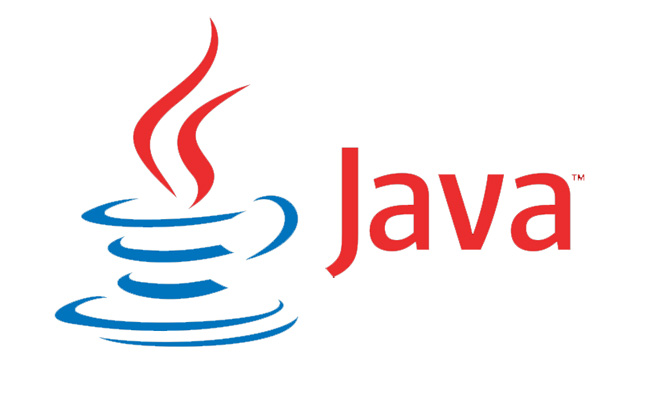
\includegraphics[width=0.3\textwidth, height=25mm]{images/java}} &
	    \begin{itemize}[topsep=0pt]
	      \item El sistema será desarrollado en lenguaje Java, debido a sus características propias del lenguaje y al conocimiento técnico que tiene de este el equipo de trabajo. Así mismo se usarán diferentes bibliotecas que probablemente auxiliarán en el desarrollo del sistema.
	      \item Las tecnologías de Java mantienen sus características de independencia de la plataforma, 
	      \item Para el desarrollo se usarán tecnologías como JSP, Object Graph Mapping (OGM).
	    \end{itemize} \cite{26}\\
	    \midrule
	    \raisebox{-\totalheight}{
\includegraphics[width=0.3\textwidth]{images/neo4j}} &
	    \begin{itemize}[topsep=0pt]
	      \item Debido a sus características como líder en la rama de las bases de datos orientadas a grafos se utilizará el sistema gestor de bases de datos proporcionado por Neo4j. 
	      \item A diferencia de los sistemas de bases de datos relacionales como MySQL, o SQL Server, las bases de datos orientadas a grafos tienen la característica de proporcionar una estructura flexible de datos, así como estar desarrollada para problemas donde las relaciones entre las entidades tienen una relevancia importante en la resolución del problema.
	    \end{itemize} \\
	    \midrule    
	    \raisebox{-\totalheight}{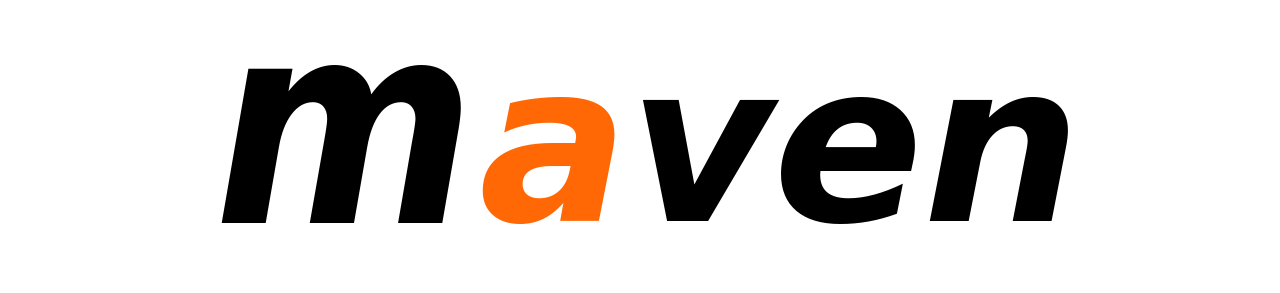
\includegraphics[width=0.3\textwidth]{images/maven}} &
	    \begin{itemize}[topsep=0pt]
	      \item Permite la construcción y gestión de proyectos Java. 
	      \item Utiliza un modelo de configuración basado XML (POM) para describir el proyecto de software a construir.
	    \end{itemize} \\
	    \bottomrule
		\end{tabular}
  	\end{center}
	\end{table}
	\begin{table}[h]
	\begin{center}
	  \begin{tabular}{ | c | p{10cm} | }
	 	% Neo4j, Java(OGM, JSP, Spring), Bootstrap, JQuery, Git
	    \toprule
	    Nombre & Ventajas \\
	    \midrule
	    \raisebox{-\totalheight}{
\includegraphics[width=0.3\textwidth]{images/jquery}} &
	    \begin{itemize}[topsep=0pt]
	      \item Es una biblioteca de JavaScript que permite simplificar la manera de interactuar con los documentos HTML.
	      \item Permite manejar eventos y agregar integración con la técnica Ajax a páginas web. 
	      \item Entre sus características podemos destacar que es una herramienta de código abierto. 
	    \end{itemize} \\
	    \midrule
	    \raisebox{-\totalheight}{
\includegraphics[width=0.3\textwidth]{images/git}} &
	    \begin{itemize}[topsep=0pt]
	      \item Es una herramienta de control de versiones (VCS) pensada en la eficiencia y la confiabilidad del mantenimiento de versiones.
	      \item Integrada con la platafroma GitHub, permite el trabajo colaborativo en diferentes proyectos.
	    \end{itemize} \\
	    \midrule
	    \raisebox{-\totalheight}{
\includegraphics[width=0.3\textwidth]{images/bootstrap}} &
	    \begin{itemize}[topsep=0pt]
	      \item Para el maquetado de las vistas, se utilizará la herramienta proporcionada por Bootstrap, que permite realizar vistas en lenjuage HTML, usando CSS y Jquery. 
	      \item Permite el desarrollo en un menor tiempo de las visas finales para proyectos web.
	    \end{itemize} \\
	    \bottomrule
		\end{tabular}
  	\caption{Descripción de las tecnologías}
  	\label{Descripción de las tecnologías}
  	\end{center}
	\end{table}
